\documentclass[border=4pt]{standalone}
\usepackage{amssymb}
\usepackage{tikz}
\usetikzlibrary{arrows.meta,positioning,shapes.geometric,fit,calc,automata,trees}
\usepackage{float}
\usepackage{booktabs}
\usepackage{longtable}
\usepackage{array}
\usepackage[utf8]{inputenc}
\begin{document}

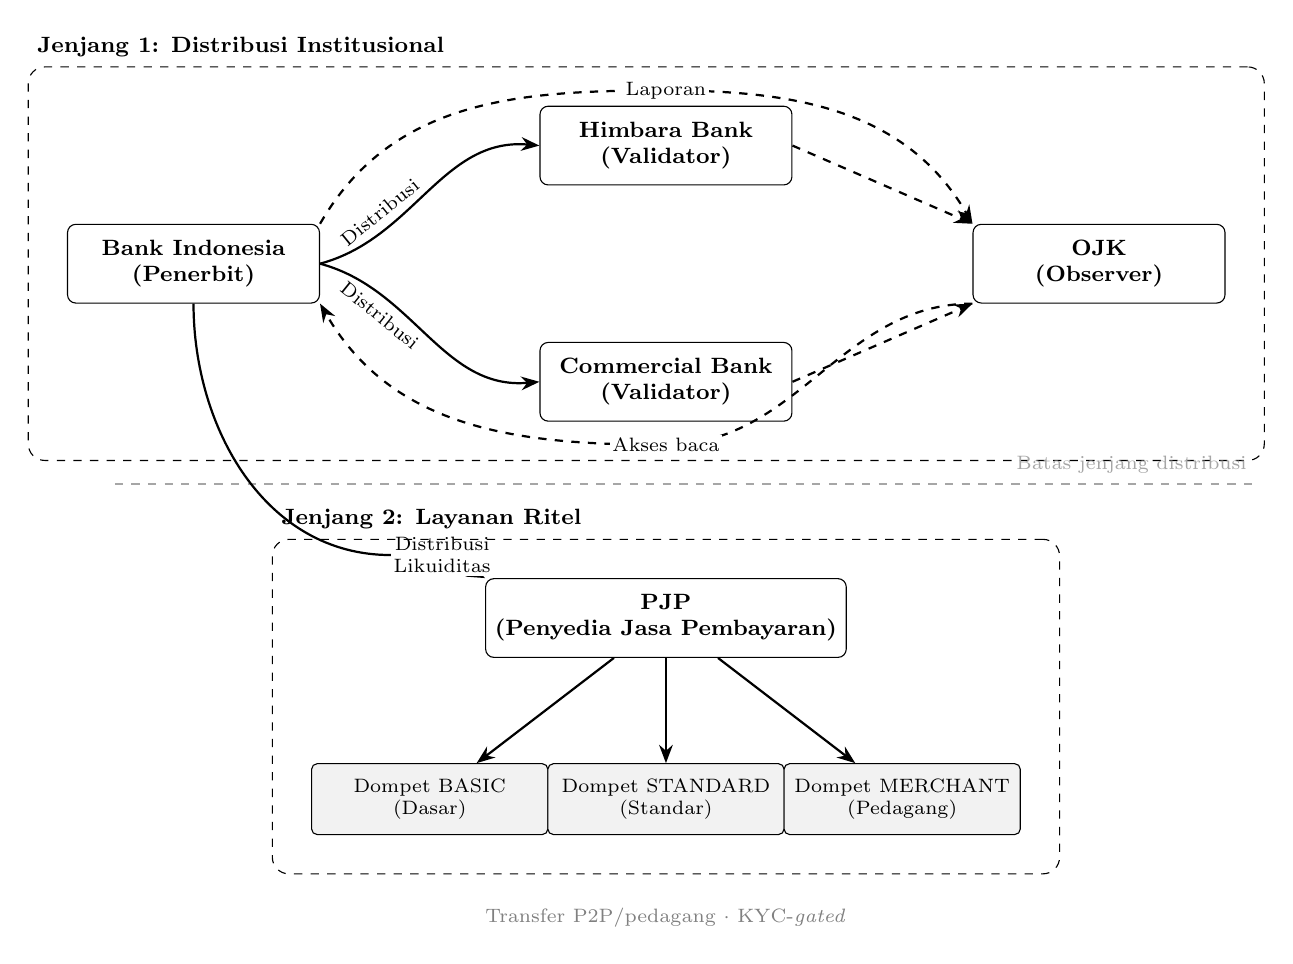
\begin{tikzpicture}[
  actor/.style={draw=black, fill=white, rectangle, rounded corners=3pt,
    minimum width=3.2cm, minimum height=1.0cm, align=center, font=\footnotesize\bfseries},
  wbox/.style={draw=black, fill=gray!10, rectangle, rounded corners=2pt,
    minimum width=3.0cm, minimum height=0.9cm, align=center, font=\scriptsize},
  zonebox/.style={draw=black, dashed, rounded corners=6pt, fill=none, inner sep=14pt},
  pl/.style={font=\scriptsize, midway, align=center},
  ar/.style={-{Stealth}, thick},
  dar/.style={-{Stealth}, thick, dashed},
]

%── Jenjang distribusi institusional ──────────────────────────────────────────

\node[actor] (bi)         at (0,    0)    {Bank Indonesia\\(Penerbit)};
\node[actor] (himbara)    at (6.0,  1.5)  {Himbara Bank\\(Validator)};
\node[actor] (commercial) at (6.0, -1.5)  {Commercial Bank\\(Validator)};
\node[actor] (ojk)        at (11.5, 0)    {OJK\\(Observer)};

% BI → Banks (penerbitan dan distribusi)
\draw[ar] (bi.east) to[out=15,in=175]
  node[pl, above, sloped, pos=0.3]{Distribusi} (himbara.west);
\draw[ar] (bi.east) to[out=-15,in=-175]
  node[pl, below, sloped, pos=0.3]{Distribusi} (commercial.west);

% Pelaporan dan akses baca pengawasan
\draw[dar] (bi.north east) to[out=60,in=180] (6.0,2.2)
  to[out=0,in=120] (ojk.north west);
\node[font=\scriptsize, align=center, fill=white, inner sep=1pt]
  at (6.0,2.2) {Laporan};
\draw[dar] (ojk.south west) to[out=180,in=0] (6.0,-2.3)
  to[out=180,in=-60] (bi.south east);
\node[font=\scriptsize, align=center, fill=white, inner sep=1pt]
  at (6.0,-2.3) {Akses baca};

% Peserta validator → OJK (pelaporan)
\draw[dar] (himbara.east)    -- (ojk.north west);
\draw[dar] (commercial.east) -- (ojk.south west);

\node[zonebox,
  fit=(bi)(himbara)(commercial)(ojk),
  label={[font=\footnotesize\bfseries, anchor=south west]north west:%
    Jenjang 1: Distribusi Institusional}] (j1) {};

%── Batas tier ────────────────────────────────────────────────────────────────

\draw[dashed, thick, gray!70] (-1.0, -2.8) -- (13.5, -2.8);
\node[font=\scriptsize, gray!70, anchor=east] at (13.5, -2.55)
  {Batas jenjang distribusi};

%── Distribusi lintas jenjang ─────────────────────────────────────────────────

\node[actor] (pjp) at (6.0, -4.5) {PJP\\(Penyedia Jasa Pembayaran)};

\draw[ar] (bi.south) to[out=-90,in=180] (2.5,-3.7)
  to[out=0,in=155] (pjp.north west);
\node[font=\scriptsize, align=center, anchor=west, fill=white, inner sep=1pt]
  at (2.5,-3.7) {Distribusi\\Likuiditas};

%── Jenjang 2: Retail ────────────────────────────────────────────────────────

\node[wbox] (tbasic)    at (3.0, -6.8) {Dompet BASIC\\(Dasar)};
\node[wbox] (tstandard) at (6.0, -6.8) {Dompet STANDARD\\(Standar)};
\node[wbox] (tmerchant) at (9.0, -6.8) {Dompet MERCHANT\\(Pedagang)};

\draw[ar] (pjp) -- (tbasic);
\draw[ar] (pjp) -- (tstandard);
\draw[ar] (pjp) -- (tmerchant);

\node[zonebox,
  fit=(pjp)(tbasic)(tstandard)(tmerchant),
  label={[font=\footnotesize\bfseries, anchor=south west]north west:%
    Jenjang 2: Layanan Ritel}] (j2) {};

\node[font=\scriptsize, gray] at (6.0, -8.3)
  {Transfer P2P/pedagang $\cdot$ KYC-\textit{gated}};

\end{tikzpicture}%

\end{document}
